% !TEX root = 6490.tex









\section{Reductive groups}

Let $k$ be an algebraically closed field of characteristic zero. Let 
$G_{/k}$ be a reductive algebraic group. That is, $G$ is connected and 
$\urad G=1$. We will associate to $G$ some combinatorial data, called the 
\emph{root datum}. The root datum of $G$ will characterize $G$ up to 
isomorphism, will not depend on the field $k$, and will completely determine 
the representation theory of $G$. Much of the theory will depend on the 
notions of \emph{maximal torus} and \emph{Borel subgroup}. To prove basic 
properties of these, we need to be able to take quotients, and it is to this 
that we now turn. The theory of quotients requires quite a bit of, 
sophistication, and may safely be skipped at first reading. 





\subsection{Quotients \texorpdfstring{$\star$}{*}}

The ``morally correct'' place to take quotients is in the category of 
fppf sheaves. 

\begin{definition}
A finite family $\{f_i:X_i\to X\}$ of morphisms of schemes is an 
\emph{fppf cover} if it is jointly surjective (on points), and each 
$X_i\to X$ is flat, of finite presentation, and quasi-finite. 
\end{definition}

We write $\fppf$ for the topology generated by fppf covers. Recall that a 
topology is called \emph{subcanonical} if each representable functor is a 
sheaf. Also, a \emph{sieve} on $X$ is a subfunctor of $h_X=\hom(-,X)$. 
We reproduce the following theorem from SGA. 

\begin{theorem}
\leavevmode
\begin{enumerate}
\item
A sieve $S$ on $X$ is a cover for the fppf topology if and only if there is 
an open affine cover $\{X_i\}$ of $X$ together with affine fppf covers 
$\{X_{i j}\to X_i\}$ such that each $X_{i j}\to X$ is in $S$. 

\item A presheaf $F$ on $\schemes{}$ is an fppf sheaf if and only if: 
  \begin{enumerate}
  \item $F$ is a Zariski sheaf.  
  \item For each fppf cover $X\to Y$, where $X$ and $Y$ are affine, the 
    following diagram is an equalizer: 
    \[\begin{tikzcd}
      F(X) \ar[r] 
        & F(Y) \ar[r, shift left=.5ex] \ar[r, shift right=.5ex]
        & F(Y\times_X Y) .
    \end{tikzcd}\]
  \end{enumerate}
  
\item The fppf topology is subcanonical. 

\item If $\{X_i\to X\}$ is jointly surjective and each $X_i\to X$ is 
faithfully flat and of finite presehtation, then $\{X_i\to X\}$ is an fppf 
cover. 
\end{enumerate}
\end{theorem}
\begin{proof}
This is \cite[IV 6.3.1]{sga3-i}. 
\end{proof}

A good general source for topologies and sheaves is the book 
\cite{maclane-moerdijk-1994}. From it, we get that the category 
$\sheaves_\fppf(\schemes S)$ is a \emph{topos}. That is, limits, colimits 
and more exist in the category of sheaves on $\schemes S$. However, it can 
be quite tricky to check whether a given colimit of schemes (taken in the 
fppf topology) is actually represented by a scheme. 

Let $k$ be a field. For the remainder, we'll work in the category of 
fppf sheaves on $\schemes k$. We'll call such sheaves \emph{spaces}. 

\begin{definition}
Let $G$ be a $k$-group space. A $k$-space $X$ is called a \emph{$G$-space} if 
it is equipped with a morphism $G\times X\to X$, such that for each 
$S\in \schemes k$, the map $G(S)\times X(S)\to X(S)$ gives an action of the 
group $G(S)$ on the set $X(S)$. 
\end{definition}

If $G_{/k}$ is an algebraic group and $X_{/k}$ is a variety, we call $X$ a 
\emph{$G$-variety}, or \emph{variety with $G$-action}. (Recall that for us, 
a \emph{variety} over $k$ is a separated scheme of finite type over $k$.) The 
representability of quotients $G\backslash X$ is a subtle one, but fortunately 
we only need to take quotients $G/H$, where $H\subset G$ is an algebraic 
subgroup. 

\begin{theorem}
Let $G_{/k}$ be an algebraic group, $H\subset G$ an algebraic subgroup. Then 
the fppf quotient $G/H$ is a variety over $k$. If $G$ is smooth, so is $G/H$, 
and if $H$ is normal, then $G/H$ has a unique structure of a group scheme for 
which $G\to G/H$ is a homomorphism. 
\end{theorem}
\begin{proof}
This is \cite[VI\textsubscript{A} 3.2]{sga3-i}. 
\end{proof}

A major theorem whose proof uses quotients is the Borel fixed point theorem. 
To state it, we need some terminology. Following \cite[II 5.4.1]{ega2}, we say 
a morphism $f:X\to Y$ of schemes is \emph{proper} if it is separated, of finite 
type, and if for all $Y'\to Y$, the induced morphism $X_{Y'}\to Y$ is closed. 
We call a variety $X_{/k}$ proper if the structure map $X\to \spectrum(k)$ is 
proper. There is a valuative criterion for properness \cite[II 7.3.8]{ega2}. 
One considers pairs $(A,K)$, where $A$ is a valuation ring with morphism 
$\spectrum(A)\to Y$, and $K$ is the field of fractions of $Y$. A morphism 
$X\to Y$ is proper if and only if for all such pairs, the map 
$X_{/Y}(A)\to X_{/Y}(K)$ is a bijection. If $f:X\to Y$ is a morphism of 
varieties over $\dC$, then by \cite[XII 3.2]{sga1}, $f$ is proper if and 
$f:X(\dC)\to Y(\dC)$ is proper in the topological sense. (Following 
\cite[I \S10.2 th.1]{bourbaki-topology-1-4}, a map $f:X\to Y$ between 
Hausdorff spaces is proper if it is closed, and the preimage of a compact 
set is compact.)

\begin{theorem}\label{thm:borel-fixed}
Let $k$ be an algebraically closed field, $G_{/k}$ a connected solvable group, 
and $X_{/k}$ a proper non-empty $G$-variety. Then $X^G\ne\varnothing$. 
\end{theorem}
\begin{proof}
We induct on the dimension of $G$. If $G$ is one-dimensional, then 
$G$ is one of $\{\Ga,\Gm\}$, so in particular neither $G$ nor any of its 
nontrivial quotients are proper. For $x\in X(k)$, let 
$G_x=\stabilizer_G(x)$. Either $G_x=G$, in which case $x\in X^G(k)$, or 
$G_x$ is finite, in which case we have an embedding $G/G_x\monic X$ given 
by $g\mapsto g x$. By passing to the closure of the image of this map, 
we may assume the image of $G/G_x$ in $X$ is dense. Thus 
$X\smallsetminus G/G_x$ is a $G$-stable finite nonempty (because $G$ 
isn't proper) variety on which $G$ acts, hence 
$X^G\supset X\smallsetminus G/G_x$. 

In the general case, choose a one-dimensional normal subgroup 
$H\subset G$. By induction, $X^H\ne\varnothing$, and by the first part of 
the proof, $X^G=(X^H)^{G/H}\ne\varnothing$. 

For a more careful proof, see \cite[18.1]{milne-iAG}. 
\end{proof}

Checking the valuative (or topological) criteria for properness can be pretty 
difficult. There is a special class of morphisms, called \emph{projective 
morphisms}, that are automatically proper. Let $S$ be a base scheme, and 
$\sE$ a quasi-coherent sheaf on $S$. Define a functor $\dP(\sE)$ on 
$\schemes S$ by 
\[
  \dP(\sE)(X) = \{(\sL,\varphi):\text{$\sL$ is invertible and }\varphi:\sE_X\epic \sL\} /\simeq .
\]
That is, $\dP(\sE)(X)$ is the set of isomorphism classes of pairs 
$(\sL,\varphi)$, where $\sL$ is a line bundle on $X$ and 
$\varphi:\sE_X\epic \sL$ is a surjection. By \cite[II 4.2.3]{ega2}, this 
functor is representable. Following \cite[II 5.5.2]{ega2}, a morphism 
$f:X\to Y$ is called \emph{projective} if it factors as 
$X\monic \dP(\sE)\epic Y$, where $\sE$ is a coherent $\sO_Y$-module, 
$X\monic \dP(\sE)$ is a closed immersion and $\dP(\sE)\epic Y$ is the 
canonical morphism. Equivalently, $X$ is isomorphic to $\proj(\sA)$ for 
some sheaf $\sA=\sA_\bullet$ of graded $\sO_Y$-algebras, which is 
generated as an $\sO_Y$-algebra by $\sA_1$, and for which $\sA_1$ is coherent. 
By \cite[II 5.5.3]{ega2}, projective morphisms are proper. In particular, 
if we work over a base field $k$, all closed subschemes of 
$\dP(V)$ for a finite-dimensional $k$-vector space $V$ are proper. 





\subsection{Centralizers, normalizers, and transporter schemes}

Here we define some constructions scheme-theoretically that will be used 
extensively in the structure theory of reductive groups. Fix a base scheme 
$S$, and let $G_{/S}$ be a group scheme. If $X,Y\subset G$ are subschemes, 
the \emph{transporter scheme} $\transporter_G(X,Y)$ and the \emph{strict 
transporter scheme} $\stricttransporter_G(X,Y)$ are given by their functors 
of points:
\begin{align*}
  \transporter_G(X,Y)(T) 
    &= \{g\in G(T): \adjoint(g)(X_T)\subset Y_T\} \\
    &= \{g\in G(T):g X(T') g^{-1}\subset Y(T')\text{ for all }T'\to T\} \\
  \stricttransporter_G(X,Y)(T) 
    &= \{g\in G(T):\adjoint(g)(X_T)=Y_T\} .
\end{align*}
Similarly, if $u,v:X\to G$ are morphisms, one defines 
\[
  \transporter_G(u,v)(T) = \{g\in G(T):\adjoint(g)\circ u_T=v_V\} .
\]
This enables us to define, for a subgroup-scheme $H\subset G$, 
\begin{align*}
  \centralizer_G(H) &= \transporter_G(H\monic G,H\monic G) && \text{(the \emph{centralizer})}\\
  \normalizer_G(H) &= \stricttransporter_G(H,H) && \text{(the \emph{normalizer})}.
\end{align*}

We reproduce the following theorem from SGA. 

\begin{theorem}
Let $k$ be a field, $G_{/k}$ a group scheme of finite type. 
\begin{enumerate}
\item If $X,Y\subset G$ are closed subschemes, then $\transporter_G(X,Y)$ and 
$\stricttransporter_G(X,Y)$ are represented by closed subschemes of $G$. 

\item If $u,v:X\to G$ are two morphisms of schemes over $k$, then 
$\transporter_G(u,v)$ is represented by a closed subscheme of $G$. 
\end{enumerate}
\end{theorem}
\begin{proof}
This is essentially \cite[VI\textsubscript{B} 6.2.5]{sga3-i}. 
\end{proof}

\begin{corollary}
Let $k$ be a field, $G_{/k}$ a group scheme of finite type, and $H\subset G$ a 
closed subgroup scheme. Then $\centralizer_G(H)$ and $\normalizer_G(H)$ are 
represented by closed subgroup schemes of $G$
\end{corollary}

Clearly $\centralizer_G(H)\subset \normalizer_G(H)$. 





\subsection{Borel subgroups}

For this section, $k$ is an algebraically closed field of characteristic 
zero. 

\begin{definition}
Let $G_{/k}$ be a linear algebraic group. A \emph{Borel subgroup} of $G$ is 
a connected solvable subgroup $B\subset G$ that is maximal with respect to 
those properties. 
\end{definition}

\begin{theorem}\label{thm:borel-conjugate}
Let $G_{/k}$ be a linear algebraic group. Then all Borel subgroups of $G$ 
are conjugate. 
\end{theorem}
\begin{proof}
Let $B_1,B_2$ be two Borel subgroups. By \cite[18.11.a]{milne-iAG}, the 
variety $G/B_1$ is proper. By \autoref{thm:borel-fixed}, the left-action 
of $B_2$ on $G/B_1$ admits a fixed point $g B_1$. One has 
$B_2\subset\adjoint(g)(B_1)$; by maximality $B_2=\adjoint(g)(B_1)$. 
\end{proof}

In general, one calls the quotient $G/B$ of $G$ by a Borel subgroup $B$ the 
\emph{flag variety} of $G$. 

\begin{example}
If $G=\GL(n)$, then by \autoref{thm:lie-kolchin}, the subgroup $B$ of 
upper-triangular matrices is a Borel subgroup. We will see that 
$G/B$ is proper. Indeed, we will work in much greater generality. Let $S$ be a 
base scheme and $\sE$ a locally free $\sO_S$-module. If $X_{/S}$ is a scheme, 
write $\sE_X$ for the pullback of $\sE$ to $X$. Write $\GL(\sE)$ for the 
functor $X\mapsto \automorphisms_{\sO_X}(\sE_X)$. This is an open subscheme of 
$\dV(\sE^\vee\otimes \sE)$, so it is representable. 

Let $n=\rank(\sE)$; for $r<n$, let $\grassmannian(\sE,r)$ be the functor given 
by 
\[
  \grassmannian(\sE,r)(X) = \{\sE_X\epic \sF:\text{$\sF$ is a locally free $\sO_X$-module of rank $r$}\} /\simeq .
\]
By \cite[ex.2]{nitsure-2005}, this is representable. note that 
$\grassmannian(\sE,1) = \dP(\sE)$, so $\grassmannian(\sE,1)$ is projective. 
More generally, for each $r$ the operation ``take $r$-th wedge power'' gives 
a closed embedding $\grassmannian(\sE,r) \monic \dP(\bigwedge^r\sE)$, so all 
the $\grassmannian(\sE,r)$ are projective. Put 
$\grassmannian(\sE)=\prod_{r<n} \grassmannian(\sE,r)$; this is 
projective via the Segre embedding \cite[II 4.3.3]{ega2}
\[
  \dP(\sE)\times \cdots \times \dP(\textstyle\bigwedge^{n-1}\sE)\monic \dP(\sE\otimes \cdots \otimes \textstyle\bigwedge^{n-1} \sE) .
\]

Suppose $\sE$ admits a descending filtration $\filtration^\bullet\sE$ such that 
each quotient $\sE_r=\sE/\filtration^r$ has rank $r$. Define a closed subgroup 
of $\GL(\sE)$ by 
\[
  B(X) = \{g\in \GL(\sE)(X):g\text{ preserves }\filtration^\bullet\} .
\]
This is a Borel subgroup of $\GL(\sE)$. We will realize the relative 
flag variety $G/B$ as a closed subscheme of $\grassmannian(\sE)$. 
If $X_{/S}$ is a scheme, a \emph{flag (relative to $\sE$)} on $X$ is a diagram 
$\sE_X=\sV_n\epic \cdots \epic \sV_0=0$ of locally free quotients of $\sE_X$, 
where each $\sV_r$ has rank $r$. Write $\sV_\bullet$ for such a flag. Define a 
functor $\flag(\sE)$ by 
\[
  \flag(\sE)(X) = \{\text{flags relative to $\sE$ on $X$}\} / \simeq .
\]
The rule $\sV_\bullet\mapsto (\sV_r)_r$ gives a closed embedding 
$\flag(\sE)\monic \grassmannian(\sE)$. See 
\cite[I \S 2 6.3]{demazure-gabriel-1980} for a proof when $S=\spectrum(\dZ)$ 
and $\sE=\dZ^n$. 

Our filtration $\filtration^\bullet\sE$ induces an element of $\flag(\sE)(S)$, 
namely $\{\sE\epic\sE/\filtration^r\}_r$. The action of $\GL(\sE)$ on $\sE$ 
induces a right action of $\GL(\sE)$ on $\flag(\sE)$, in which an 
element $g\in \GL(\sE)(X)$ acts on a flag $\sE\epic \sV_\bullet$ by 
$\sE\xrightarrow g \sE\epic \sV_\bullet$. Moreover, $B\subset \GL(\sE)$ 
acts trivially. Assume $S$ is locally noetherian. Then by 
\cite[V 10.1.1]{sga3-i}, the quotient $\GL(\sE)/B$ exists and comes with 
an embedding $\GL(\sE)/B\monic \flag(\sE)$. We claim that this map is 
surjective, hence an isomorphism. Indeed, Zariski-locally, it comes down to 
checking that $\GL(A^n)/B(A)\to \flag(A^n)$ is surjective, which is a basic 
fact from linear algebra. Thus $\GL(\sE)/B\iso \flag(\sE)$. 
\end{example}

We will be mainly interested in when $S=\spectrum(k)$ and 
$V=k^n$. In this case, we write $\grassmannian(n,r)=\grassmannian(k^n,r)$ 
and $\flag(n)=\flag(k^n)$. Thus $\GL(n)/B\iso \flag(n)\monic \grassmannian(n)$. 
More generally, we have the following fact. 

\begin{theorem}
Let $G$ be a linear algebraic group, $B\subset G$ a Borel subgroup. Then 
$G/B$ is a projective variety. 
\end{theorem}

\begin{definition}
Let $G$ be a linear algebraic group. A closed subgroup $P\subset G$ is 
\emph{parabolic} if $G/P$ is proper. 
\end{definition}

\begin{theorem}
A subgroup $P\subset G$ is parabolic if and only if $P$ contains a Borel 
subgroup of $G$. 
\end{theorem}
\begin{proof}
$\Leftarrow$. Suppose $P$ contains a Borel subgroup $B$. Then the inclusion 
$B\subset P$ induces a map $G/B\epic G/P$. Since $G/B$ is proper, by 
\cite[II 5.4.3]{ega2}, so is $G/P$. Alternatively, see \cite[XVI 2.5]{sga3-ii} 
for a proof over a general base. 

$\Rightarrow$. Consider the action of $B$ on the proper variety $G/P$. 
By \autoref{thm:borel-fixed}, there is a fixed point $g P$. One obtains 
$\adjoint(g^{-1})(B)\subset P$, so $P$ contains a Borel subgroup. 
\end{proof}

In light of this result, we could have defined a Borel subgroup to be a minimal 
parabolic subgroup. 





\subsection{Maximal tori}

For this section, $k$ is an algebraically closed field of characteristic 
zero. Let $G_{/k}$ be a linear algebraic group. A \emph{maximal torus} in 
$G$ is a subgroup scheme $T\subset G$ that is a torus, and is maximal with 
respect to this property. In our setting, any torus in $G$ is contained in a 
maximal torus. 


\begin{example}
Let $G=\GL(n)$. Then we can choose $T$ to be the subgroup consisting of 
diagonal matrices. This is a maximal torus because all tori are diagonalizable, 
so any torus in $\GL(n)$ is conjugate to a subgroup of $T$. A Borel subgroup 
consists of upper-triangular matrices. 
\end{example}

\begin{theorem}
Let $G_{/k}$ be a linear algebraic group. Then all maximal tori are conjugate. 
\end{theorem}
\begin{proof}
If $G$ is solvable, this is \cite[17.40]{milne-iAG}. Essentially, one uses 
the fact that $G=T\ltimes \urad G$ for any maximal torus $T$. 

If $G$ is a general group, then different maximal tori $T_1,T_2$ will live in 
Borel subgroups $B_1,B_2$. By \autoref{thm:borel-conjugate}, the subgroups 
$B_1$ and $B_2$ are conjugate, so we may as well assume $T_1$ and $T_2$ are 
maximal tori in the same Borel subgroup $B$. But then we can use the fact that 
the theorem holds for solvable groups. 
\end{proof}

\begin{example}
Let $\rho:G\to \GL(V)$ be a representation, where $G$ is a connected 
solvable group. Then $G$ acts on $\dP(V)$ via $\GL(V)$, so 
\autoref{thm:borel-fixed} tells us that $G$ fixes a vector, i.e.~that 
$V$ contains a $G$-invariant line. 
\end{example}

\begin{lemma}
Let $T\subset G$ be a torus. Then the quotient 
$\weyl_G(T)=\centralizer_G(T)^\circ=\normalizer_G(T)^\circ$, hence the quotient 
$\normalizer_G(T)/\centralizer_G(T)$ is finite \'etale. 
\end{lemma}
\begin{proof}
There is an obvious family $\normalizer_G(T)^\circ\times T\to T$ given by 
$(y,t)\mapsto y t y^{-1}$. By \autoref{thm:rigidity-tori}, this is constant, 
hence $\normalizer_G(T)^\circ\subset \centralizer_G(T)$. 
\end{proof}

One calls $\weyl_G(T)$ the \emph{Weyl group} of the pair $(G,T)$. It is finite 
\'etale over $k$. 

\begin{lemma}
Let $G_{/k}$ be a connected reductive group. Then $\rad G=\zentrum(G)^\circ$. 
\end{lemma}
\begin{proof}
Note that $\rad G$ is a torus. Since $\rad G$ is normal in $G$, there is a 
family $G\times \rad G\to \rad G$ given by $(y,t)\mapsto y t y^{-1}$. Again 
by \autoref{thm:rigidity-tori}, this is trivial, hence 
$\rad G\subset \zentrum(G)$. The result follows. 
\end{proof}

\begin{lemma}\label{lem:semisimple-reductive}
Let $G$ be a connected linear algebraic group that admits a faithful 
irreducible representation $\rho:G\monic \GL(V)$. Then $G$ is reductive. 
\end{lemma}
\begin{proof}
We may assume that $G\subset \GL(V)$. Let $H=\urad G$; the space $V^H$ is 
nonzero since $H$ is unipotent. In fact, since $H$ is normal in $G$, 
$V^H$ is a subrepresentation of $V$. Since $V$ is simple, $V^H=V$. But 
$G\subset \GL(V)$, so $H=1$. 
\end{proof}

\begin{corollary}
The groups $\GL(n)$, $\SL(n)$, $\SO(2n)$ and $\Sp(2n)$ are reductive. 
\end{corollary}
\begin{proof}
Apply \autoref{lem:semisimple-reductive} to the standard representations. For 
$\SO$ and $\Sp$, use the fact that the group preserves a nondegenerate bilinear 
form. 
\end{proof}





\subsection{Root systems}

Let $k$ be a field, $G_{/k}$ a reductive group, $\fg=\lie(G)$. In 
\autoref{sec:lie-alg-of-group}, we defined a canonical representation 
$\adjoint:G\to \GL(\fg)$. Let $T\subset G$ be a maximal torus. We are 
interested in the representation $\adjoint|_T:T\to \GL(\fg)$. For simplicity, 
assume $T$ is diagonalizable (i.e.~, a \emph{split} torus). By 
\autoref{thm:diag-groups}, there is a decomposition 
\[
  \fg = \bigoplus_{\alpha\in\characters^\ast(T)} \fg_\alpha ,
\]
where for $\alpha\in \characters^\ast(T)$, the space 
$\fg_\alpha=\{x\in \fg:t g=\alpha(t) g\text{ for all }t\in T\}$. Let 
$\roots(G,T) = \{\alpha\in \characters^\ast(T)\smallsetminus 0:\fg_\alpha\ne 0\}$. 
Then we tautologically have a decomposition 
\[
  \fg=\fg_0\oplus \bigoplus_{\alpha\in \roots(G,T)} \fg_\alpha .
\]
We call $\roots(G,T)\subset \characters^\ast(G)$ the set of \emph{roots} of 
$G$. This is a finite set. 

Let $V$ be the span of $\roots(G,T)$ in 
$\characters^\ast(T)_\dR=\characters^\ast(T)\otimes\dR$. The finite set 
$\roots(G,T)$ sitting inside the real vector space $V$ is an example of a 
``root system.'' General root systems break up into irreducibles, and there is 
a combinatorial classification of irreducible root systems into 
types 
$\typeA_n,\typeB_n,\typeC_n,\typeD_n,\typeG_2,\typeF_4,\typeE_6,\typeE_7,\typeE_8$. 
The root datum $\roots(G,T)\subset V$ will recover $G/\zentrum(G)$. 





\begin{example}
We will work out the root datum of $\SL(n+1)$ for $n\geqslant 1$. We choose 
the maximal torus 
\begin{align*}
  T &= \left\{\diagonal(a_1,\dots,a_{n+1}):a_i\in \Gm\text{ and }\prod a_i=1\right\} \\
  &= \begin{pmatrix} \ast \\ & \ddots \\ & & \ast \end{pmatrix} \subset \SL(n+1) .
\end{align*}
Define $\chi_i:T\to \Gm$ by $\chi_i(\diagonal(a_1,\dots,a_{n+1}))=a_i$. Then 
$(\chi_1,\dots,\chi_n)$ induces an isomorphism between $T$ and the subgroup of 
$\Gm^{n+1}$ consisting of $(a_1,\dots,a_{n+1})$ with $a_1\dotsm a_{n+1})=1$. 
Thus $\characters^\ast(T)=\{\sum a_i \chi_i:\sum a_i=0\}$. 

The Lie algebra $\Sl(n+1)$ is spanned by $\ft=\lie(T)$ and the set 
\[
  \left\{E_{i,j} = (\delta_{i,a}\delta_{j,b})_{a,b}\right\} \subset \Sl(n+1) .
\]
Moreover, one can check that 
\[
  \adjoint\left(\diagonal(a_1,\dots,a_{n+1})\right)(E_{i,j}) = \frac{a_i}{a_j} E_{i,j} .
\]
Thus, the root decomposition of $\Sl(n+1)$ is 
\[
  \Sl(n+1) = \ft\oplus \bigoplus_{i\ne j} \langle E_{i,j}\rangle .
\]
So $\roots(\SL_{n+1},T) = \{\chi_i-\chi_j:i\ne j\}$. We think 
of $\roots(\SL_{n+1})$ as a subset of the real vector space 
$\{\sum a_i \chi_i:a_i\in \dR\text{ and }\sum a_i=0\}$. 
\end{example}

With this example in mind, we move towards the general definition of a root 
system. Fix a finite-dimensional $\dR$-vector space $V$. For 
$\alpha\in V\smallsetminus 0$, a \emph{reflection} on $V$ with vector $\alpha$ 
is a linear map $s:V\to V$ such $s(\alpha)=-\alpha$, and for which there exists 
a decomposition $V=\dR\alpha\oplus U$ such that $\alpha|_U=1$. Note that if 
$s$ is a reflection with vector $\alpha$, then $s(v)-v\in \dR\alpha$ for all 
$v\in V$. 

\begin{lemma}
Let $V$ be a finite-dimensional $\dR$-vector space, $R\subset V$ a finite 
set which spans $V$, and $\alpha\in V\smallsetminus 0$. There exists at most 
one reflection $s$ of $V$ with vector $\alpha$ such that $s(R)=R$. 
\end{lemma}
\begin{proof}
This is \cite[VI \S 1.1 lem.1]{bourbaki-lie-alg-4-6}. 
Suppose $s,s'$ are two such reflections. Define $u=s (s')^{-1}$. Note that 
$u(\alpha)=\alpha$. Moreover, $u$ induces the identity on $V/\alpha$. This 
implies $u$ is unipotent. But $u(R)=R$, so $u^n=1$ for some $n\geqslant 1$. 
This means that $u$ is semisimple. The only way an operator can be both 
unipotent and semisimple is for $u=1$. 
\end{proof}

\begin{definition}
Let $V$ be a finite-dimensional $\dR$-vector space. A subset 
$R\subset V\smallsetminus 0$ is a \emph{root system} in $V$ if the following 
hold:
\begin{enumerate}
  \item $R$ is finite and spans $V$. 
  \item For each $\alpha\in R$, there is a (unique) reflection $s_\alpha$ with 
    vector $\alpha$ such that $s_\alpha(R) = R$. 
  \item For each $\alpha,\beta\in R$, $s_\alpha(\beta)-\beta\in \dZ\alpha$. 
\end{enumerate}
\end{definition}

Often, we will speak of ``a root system $R$,'' and tacitly assume that the 
vector space $V$ has been given. One calls the elements of $R$ \emph{roots} 
of $R$. 

Let $R\subset V$ be an arbitrary root system. For any root $\alpha\in R$, the 
reflection $s_\alpha$ acts on $\alpha$ by $-1$, that is, 
$s_\alpha(\alpha)=-\alpha$. Thus $\alpha\in R\Rightarrow -\alpha\in R$. 

\begin{definition}
A root system $R$ is \emph{reduced} if whenever $c\alpha\in R$ for some 
$c\in \dR$, $\alpha\in R$, then $c=\pm 1$. 
\end{definition}

\begin{definition}
Let $R$ be a root system. The \emph{Weyl group} of $R$ is the subgroup 
$W=\weyl(R)$ of $\GL(V)$ generated by $\{s_\alpha:\alpha\in R\}$. 
\end{definition}

Since each $s_\alpha$ preserves $R$, the group $W$ preserves $R$. Moreover, 
since $R$ spans $V$, an element $w\in W$ is determined by its restriction 
$w|_R\in \permutations(R)$. Thus $W\monic \permutations(R)$, so $W$ is finite 
with cardinality $\leqslant (\# R)!$. 

For an arbitrary root system $R\subset V$, there always exists a nondegenerate 
inner product $\langle\cdot,\cdot\rangle:V\times V\to \dR$ that is 
$W$-invariant in the sense that $\langle w u,w v\rangle = \langle u,v\rangle$ 
for all $w\in W$. Existence of such an inner product follows from the 
``unitary trick.'' If $G$ is an arbitrary compact group acting continuously 
on a Hilbert space $V$, define a new inner product by 
\[
  \langle u,v\rangle_G = \int_G \langle g u,g v\rangle\, \mathrm{d} g .
\]
Then $\langle\cdot,\cdot\rangle_G$ is $G$-invariant. 

Fix a $W$-invariant inner product $\langle\cdot,\cdot\rangle$ on $V$. For 
$\alpha\in R$, we can write $V=\dR\alpha\oplus (\dR\alpha)^\bot$. One has 
\[
  s_\alpha(v) = v-2\frac{\langle v,\alpha\rangle}{\langle \alpha,\alpha\rangle} \alpha .
\]
Condition 3 in the definition of a root system comes down to requiring that 
$2\frac{\langle \beta,\alpha\rangle}{\langle \alpha,\alpha\rangle}\in \dZ$ for 
all $\alpha,\beta\in R$. For the remainder, put 
$n(\beta,\alpha) = 2\frac{\langle \beta,\alpha\rangle}{\langle \alpha,\alpha\rangle}$. 

\begin{example}
Let $V=\dR$, and $R=\{\pm \alpha\}$ for some $\alpha\ne 0$. This is the unique 
one-dimensional reduced root system, up to isomorphism. 
\end{example}

\begin{definition}
Let $R_1\subset V_1$, $R_2\subset V_2$ be root systems. The \emph{direct sum 
of $R_1$ and $R_2$} has vector space $V_1\oplus V_2$, with root system 
$\{R_1\times 0\}\sqcup \{0\times R_2\}$. 
\end{definition}

We call a root system \emph{reducible} if it can be written as the direct sum 
of two nonzero root systems, and \emph{irreducible} otherwise. From 
\cite[VI \S 1.2 prop.5]{bourbaki-lie-alg-4-6}, we see that a root system 
$R\subset V$ is reducible if and only if $V$ is reducible as a $W$-module. 
Moreover, the decomposition of a root system into irreducibles is determined by 
the decomposition of $V$ into irreducible $W$-modules. 

\begin{definition}
A subset $S\subset R$ is a \emph{base} if 
\begin{enumerate}
  \item $S$ is a basis of $V$
  \item For any $\beta\in R$, write $\beta=\sum_{\alpha\in S} m_\alpha \alpha$. 
    Then either all $m_\alpha\geqslant 0$ or all $m_\alpha\leqslant 0$. 
\end{enumerate}
\end{definition}

Let $S\subset R$ be a base; one calls the $\alpha\in S$ \emph{simple roots}. 
Let $R^+\subset R$ be the collection of $\beta\in R$ such that in the 
decomposition $\beta=\sum_{\alpha\in S} m_\alpha \alpha$, one has all 
$m_\alpha\geqslant 0$. If we put $R^-=-R^+$, then by 
\cite[VI \S 1.6 th.3]{bourbaki-lie-alg-4-6}, one has 
$R=R^+\sqcup R^-$. 

\begin{theorem}
Let $R$ be a root system. 
\begin{enumerate}
\item A base for $R$ exists. 
\item If $S_1,S_2\subset R$ are bases, then there exists $w\in W$ such that 
$w(S_1)=S_2$. 
\item $R=\bigcup_{w\in W} w(S)$. 
\item $W$ is generated by $\{s_\alpha:\alpha\in S\}$. 
\end{enumerate}
\end{theorem}
\begin{proof}
These all follow from various results in 
\cite[VI \S 1.5]{bourbaki-lie-alg-4-6}. Namely, 1 and 4 follow from parts 
(ii) and (vii) of Theorem 2. The claim 3 follows from Proposition 15, and 2 
follows from the corollary to that proposition. 
\end{proof}

Let $R\subset V$ be a reduced root system, $W=\weyl(R)$, and 
$\langle\cdot,\cdot\rangle$ a $W$-invariant inner product on $V$. Fix 
$\alpha,\beta\in R$ that are linearly independent. Let $\phi$ be the angle 
between $\alpha$ and $\beta$, determined by 
$\langle \alpha,\beta\rangle = |\alpha|\cdot |\beta| \cos\phi$. We have 
$n(\beta,\alpha)=2\frac{|\beta|}{|\alpha|}\cos\phi\in \dZ$. Moreover, 
$n(\alpha,\beta)n(\beta,\alpha)=4\cos^2\phi\in \{0,1,2,3,4\}$, so the 
possibilities for $\phi$ are very limited. In fact, we can write them all 
down:  
\begin{center}
\begin{tabular}{c|c|c|c}
  $n(\alpha,\beta)$ & $n(\beta,\alpha)$ & $\phi$ & $|\beta|/|\alpha|$ \\ \hline 
  $0$  & $0$  & $\pi/2$  & ? \\
  $1$  & $1$  & $\pi/3$  & $1$ \\
  $-1$ & $-1$ & $2\pi/3$ & $1$ \\
  $1$  & $2$  & $\pi/4$  & $\sqrt 2$ \\
  $-1$ & $-2$ & $3\pi/4$ & $\sqrt 2$ \\
  $1$  & $3$  & $\pi/6$  & $\sqrt 3$ \\
  $-1$ & $-3$ & $5\pi/6$ & $\sqrt 3$
\end{tabular}
\end{center}

Even with this finite list, classifying reduced root systems directly is 
tricky. We will classify them via a type of graph (with extra data) called a 
\emph{Dynkin diagram}. The following definition is from 
\cite[VI \S 4.2]{bourbaki-lie-alg-4-6}.

\begin{definition}
A \emph{Dynkin graph} is a pair $(\Gamma,f)$, where $\Gamma$ is an 
undirected graph and 
\[
  f:\{(\gamma_1,\gamma_2)\in \Gamma\times\Gamma:\text{$\gamma_1$ and $\gamma_2$ are connected by an edge}\}\to \dR 
\]
satisfies $f(\gamma_1,\gamma_2)f(\gamma_2,\gamma_1)=1$ whenever the expression 
is defined. 
\end{definition}

If $R\subset V$ is a reduced root system, we define a Dynkin graph 
$(Df),=\dynkin(R)$ as follows. Choose a base $S$ of $R$. The vertices of $D$ 
are elements of $S$. Given $\alpha\ne\beta\in S$, put 
$f(\alpha,\beta)=\frac{n(\alpha,\beta)}{n(\beta,\alpha)}$. For any two 
vertices $\alpha,\beta\in R$, after possibly switching $\alpha$ and 
$\beta$, we will have $f(\alpha,\beta)\in \dZ$. In $\dynkin(R)$, there are 
$|f(\alpha,\beta)$ edges between $\alpha$ and $\beta$. From the above table, 
we see that there are at most $3$ edges. 

By \cite[VI \S 4.2]{bourbaki-lie-alg-4-6}, the Dynkin diagram $\dynkin(R)$ 
only depends on $R$, in the sense that the choice of another basis yields a 
Dynkin graph that is canonically isomorphic to the first one. Moreover, 
$\dynkin(-)$ induces an injection from the set of isomorphism classes of 
reduced root systems to the set of isomorphism classes of Dynkin graphs. 
Moreover, $R$ is irreducible if and only if $\dynkin(R)$ is connected, the 
decomposition of $R$ into irreducibles matches the decomposition of 
$\dynkin(R)$ into connected components, and 
$\automorphisms(R)/\weyl(R)\iso \automorphisms(\dynkin R)$. 





\subsection{Classification of root systems}

We begin with what will turn out to be a complete list of examples of reduced 
root systems, following \cite[VI \S4]{bourbaki-lie-alg-4-6}. For some of the 
more complicated root systems (e.g.~$\typeE_8$) we only give the associated 
Dynkin diagram. When drawing Dynkin diagrams, if $f(i,j)>1$, we place an 
inequality sign $>$ over the arrows from $i$ to $j$. For example, if 
$f(i,j)=2$, we put $i\Rightarrow j$. 


\begin{example}[type $\typeA_n$, $n\geqslant 1$]
Let $n\geqslant 1$. Let $V=\{x\in \dR^{n+1}:\sum x_i=0\}$, and give $\dR^{n+1}$ 
the standard basis $e_1,\dots,e_{n+1}$ and standard inner product 
$\langle\cdot,\cdot\rangle$. The root system $\typeA_n\subset V$ is 
\[
  \typeA_n=\{e_i-e_j:i\ne j\} .
\]
Clearly $\typeA_n$ is finite and spans $V$. For each root $\alpha$, put 
\[
  s_\alpha(v) = v-2\frac{\langle v,\alpha\rangle}{\langle \alpha,\alpha\rangle} \alpha  = v-\langle v,\alpha\rangle \alpha .
\]
If $i<j$, then it is easy to check that 
\[
  s_{e_i-e_j}(a_1,\dots,a_{n+1}) = (a_1,\dots,a_j,\dots,a_i,\dots,a_{n+1}) \qquad \text{($a_i$ and $a_j$ swapped)}
\]
For all $\alpha,\beta\in \typeA_n$, one has 
$s_\alpha(\beta)-\beta=-\langle \beta,\alpha\rangle\alpha$, and 
$\langle \beta,\alpha\rangle\in \{0,\pm 1,\pm 2\}$, so $\typeA_n$ is indeed 
a root system. It is clearly reduced. The group $\weyl(\typeA_n)$ is generated 
by all linear transformations of the form ``swap $i$th and $j$th coordinates.'' 
Thus we can identify $\weyl(\typeA_n)$ with the set of permutation matrices 
in $\GL(V)$. Note that the standard inner product $\langle\cdot,\cdot\rangle$ 
on $V$ is $W$-invariant. 
\end{example}

\begin{example}[type $\typeA_1\times \typeA_1$]
This root system lives inside $V=\dR^2$ and 
$R=\{\pm (\alpha,0),\pm (0,\beta)\}$. We draw it as: 
\begin{center}
\begin{tikzpicture}[>=latex]
\draw[blue,dashed] (-1.5,0) -- (1.5,0);
\draw[blue,dashed] (0,-1.5) -- (0,1.5);
\draw[black,thick,->] (0,0) -- (0,1) node[right] {\(\alpha\)};
\draw[black,thick,->] (0,0) -- (0,-1) node[right] {\(-\alpha\)};
\draw[black,thick,->] (0,0) -- (1,0) node[above] {\(\beta\)};
\draw[black,thick,->] (0,0) -- (-1,0) node[above] {\(-\beta\)};
\end{tikzpicture}
\end{center}
The Dynkin diagram of $\typeA_1\times \typeA_1$ is a disjoint union of 
two points. 
\end{example}


\begin{example}[type $\typeA_2$]
This root system can be drawn as living in $\dR^2$ with the standard metric. It 
looks like:
\begin{center}
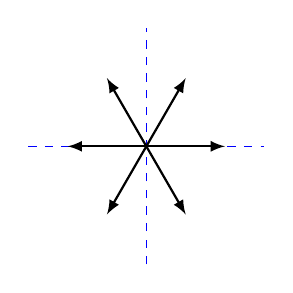
\begin{tikzpicture}[>=latex]
\draw[blue,dashed] (-1.5,0) -- (1.5,0);
\draw[blue,dashed] (0,-1.5) -- (0,1.5);
\foreach \k in {1,...,6} {
  \draw[black,thick,->](0,0) -- +(\k * 60:1);
}
\end{tikzpicture}
\end{center}
The roots lie on the unit circle and at multiples of the angle $\pi/3$. 
The Dynkin diagram is 
$\begin{tikzcd} \bullet \ar[r, dash] & \bullet \end{tikzcd}$. 
\end{example}

\begin{example}[type $\typeB_n$, $n\geqslant 2$]
Let $V=\dR^n$ and the roots be $\{\pm e_i\}\cup \{\pm e_i\pm e_j:i<j\}$. The 
Dynkin diagram of $\typeB_n$ is 
\[
\begin{tikzcd}
  \bullet \ar[r, dash] 
    & \bullet \ar[r, dash] 
    & \cdots \ar[r, dash] 
    & \bullet \ar[r, dash] 
    & \bullet \ar[r, Rightarrow] 
    & \bullet 
\end{tikzcd}
\qquad\text{($n$ vertices)} .
\]
\end{example}

\begin{example}[type $\typeB_2$]
This root system lives in $\dR^2$, and looks like 
\begin{center}
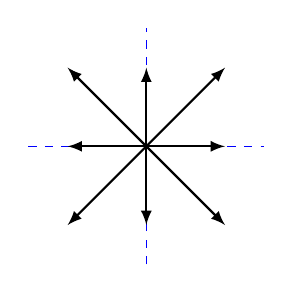
\begin{tikzpicture}[>=latex]
\draw[blue,dashed] (-1.5,0) -- (1.5,0);
\draw[blue,dashed] (0,-1.5) -- (0,1.5);
\foreach \k in {1,...,4} {
  \draw[black,thick,->] (0,0) --+(\k*90:1);
}
\foreach \k in {1,...,4} {
  \draw[black,thick,->] (0,0) --+(\k*90 + 45:{sqrt(2)});
}
\end{tikzpicture}
\end{center}
The Dynkin diagram $\dynkin(\typeB_2)$ is 
$\begin{tikzcd}\bullet \ar[r, Rightarrow] & \bullet \end{tikzcd}$. 
\end{example}

\begin{example}[type $\typeC_n$, $n\geqslant 2$]
The ambient vector space is $V=\dR^n$, and the set of roots is 
$\{\pm 2e_i\}\cup \{\pm e_i\pm e_j:i<j\}$. The Dynkin diagram is 
\[
\begin{tikzcd}
  \bullet \ar[r, dash] 
    & \bullet \ar[r, dash] 
    & \cdots \ar[r, dash] 
    & \bullet \ar[r, dash] 
    & \bullet \ar[r, Leftarrow] 
    & \bullet 
\end{tikzcd}
\qquad\text{($n$ vertices)} .
\]
\end{example}

\begin{example}[type $\typeD_n$, $n\geqslant 4$]
The ambient vector space is $V=\dR^n$, and the set of roots is 
$\{e_i\}\cup \{\pm e_i\pm e_j:i<j\}$. The Dynkin diagram is 
\[
\begin{tikzcd}
  & & & & \bullet \\
  \bullet \ar[r, dash]
    & \bullet \ar[r, dash] 
    & \cdots \ar[r, dash]
    & \bullet \ar[r, dash]
    & \bullet \ar[r, dash] \ar[u, dash] 
    & \bullet
\end{tikzcd}
\qquad\text{($n$ vertices)} .
\]
\end{example}

\begin{example}[type $\typeE_6$]
The space $V$ is the subspace of $\dR^8$ consisting of vectors $x$ such that 
$x_6=x_7=-x_8$. The roots are $\{\pm e_i\pm e_j:i<j\leqslant 5\}$, together 
with all 
\[
  \pm \frac 1 2\left(e_8-e_7-e_6 + \sum_{i=1}^5 (-1)^{\nu(i)} e_i\right) ,
\]
where $\sum \nu(i)$ is even. The Dynkin diagram is 
\[\begin{tikzcd}
  & & \bullet \\
  \bullet \ar[r, dash] 
    & \bullet \ar[r, dash]
    & \bullet \ar[r, dash] \ar[u, dash]
    & \bullet \ar[r, dash] 
    & \bullet 
\end{tikzcd}\]
\end{example}

\begin{example}[type $\typeE_7$]
Here $V$ is the hyperplane in $\dR^8$ orthogonal to $e_7+e_8$. The set of 
roots is $\{\pm e_i\pm e_j:i<j\leqslant 6\}\cup\{\pm (e_7-e_8)\}$, together 
with all 
\[
  \pm \frac 1 2\left(e_7-e_8+\sum_{i=1}^6 (-1)^{\nu(i)} e_i\right) ,
\]
where $\sum \nu(i)$ is odd. The Dynkin diagram is 
\[\begin{tikzcd}
  & & & \bullet \\
  \bullet \ar[r, dash] 
    & \bullet \ar[r, dash]
    & \bullet \ar[r, dash]
    & \bullet \ar[r, dash] \ar[u, dash]
    & \bullet \ar[r, dash] 
    & \bullet 
\end{tikzcd}\]
\end{example}

\begin{example}[type $\typeE_8$]
The vector space is $\dR^8$, and the set of roots consists of 
$\{\pm e_i\pm e_j:i<j\}$, together with all 
$\frac 1 2 \sum_{i=1}^8 (-1)^{\nu(i)} e_i$ for which $\sum \nu(i)$ is even. The 
Dynkin diagram is 
\[\begin{tikzcd}
  & & & & \bullet \\
  \bullet \ar[r, dash] 
    & \bullet \ar[r, dash]
    & \bullet \ar[r, dash]
    & \bullet \ar[r, dash]
    & \bullet \ar[r, dash] \ar[u, dash]
    & \bullet \ar[r, dash] 
    & \bullet 
\end{tikzcd}\]
\end{example}

\begin{example}[type $\typeF_4$]
The space is $\dR^4$, the set of roots is 
$\{\pm e_i\}\cup \{\pm e_i\pm e_j:e<i\}$, together with 
$\frac 1 2(\pm e_1\pm e_2\pm e_3\pm e_4)$. The Dynkin diagram is 
\[\begin{tikzcd}
  \bullet \ar[r] 
    & \bullet \ar[r, Rightarrow] 
    & \bullet \ar[r] 
    & \bullet
\end{tikzcd}\]
\end{example}

\begin{example}[type $\typeG_2$]
This is one of the exceptional root systems. It lives inside $\dR^2$ and looks 
like:
\begin{center}
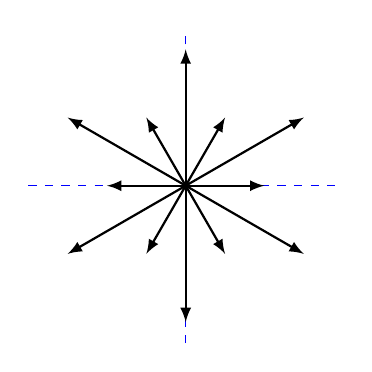
\begin{tikzpicture}[>=latex]
\draw[blue,dashed] (-2,0) -- (2,0);
\draw[blue,dashed] (0,-2) -- (0,2);
\foreach \k in {1,...,6} {
  \draw[black,thick,->](0,0) -- +(\k * 60:1);
}
\foreach \k in {1,...,6} {
  \draw[black,thick,->](0,0) -- +(\k * 60+30:{sqrt(3)});
}
\end{tikzpicture}
\end{center}
The inner collection of roots is a copy of $\typeA_2$. The outer collection 
has radius $\sqrt 3$, and is rotated by $\pi/6$. The Dynkin diagram of 
$\typeG_2$ is $\bullet \Rrightarrow \bullet$. 
\end{example}

It is possible to classify the Dynkin diagrams of irreducible reduced root 
systems. 

\begin{theorem}
Let $R$ be an irreducible reduced root system, $D=\dynkin(R)$. Then $D$ is a 
unique one of: 
\begin{itemize}
  \item $\typeA_n$ ($n\geqslant 1$)
  \item $\typeB_n$ ($n\geqslant 2$)
  \item $\typeC_n$ ($n\geqslant 3$)
  \item $\typeD_n$ ($n\geqslant 4$)
  \item $\typeE_6$, $\typeE_7$, $\typeE_8$
  \item $\typeF_4$
  \item $\typeG_2$
\end{itemize}
\end{theorem}
\begin{proof}
This is \cite[VI \S 4.2 th.3]{bourbaki-lie-alg-4-6}. 
\end{proof}

From the examples in \cite[Ch.23]{milne-iAG}, we see that we can obtain all 
the infinite families of root systems from algebraic groups:
\begin{center}
\begin{tabular}{c|c}
  group & root system \\ \hline
  $\SL(n+1)$  & $\typeA_n$ \\
  $\SO(2n+1)$ & $\typeB_n$ \\
  $\Sp(2n)$   & $\typeC_n$ \\
  $\SO(2n)$   & $\typeD_n$ 
\end{tabular}
\end{center}

Automorphisms of a reductive group will be classified by automorphisms of the 
corresponding root system. So we will make use of the following table:
\begin{center}
\begin{tabular}{c|c}
  root system                 & outer automorphisms \\ \hline
  $\typeA_1$                  & $1$ \\
  $\typeA_n$ ($n\geqslant 2$) & $\dZ/2$  \\
  $\typeB_n$                  & $1$ \\
  $\typeC_n$                  & $1$ \\
  $\typeD_4$                  & $S_3$ \\
  $\typeD_n$ ($n\geqslant 5$) & $\dZ/2$ \\
  $\typeE_6$                  & $\dZ/2$ \\
  $\typeE_7$, $\typeE_8$, $\typeF_4$, $\typeG_2$ & $1$
\end{tabular}
\end{center}




